\documentclass{amsart}
%\documentclass[a4paper,10pt]{scrartcl}

\usepackage[utf8x]{inputenc}
\usepackage[british]{babel}
%\usepackage[a4paper, inner=0.5cm, outer=0.5cm, top=1cm,
%bottom=1.5cm, bindingoffset=1cm]{geometry}
\usepackage{amsmath}
\usepackage{amssymb, latexsym}
\usepackage{longtable}
\usepackage[table]{xcolor}
\usepackage{textcomp} 
\usepackage{stmaryrd}
\usepackage{graphicx}
\usepackage{enumitem}
\usepackage{yfonts}
\usepackage{algpseudocode}
\usepackage{algorithm}
\usepackage{hyperref}
\usepackage{MnSymbol}

\setlist[enumerate]{label*=\arabic*.}
\newtheorem{theorem}{Theorem}[section]
\newtheorem{example}{Example}[section]
\newtheorem{definition}{Definition}[section]
\newtheorem{proposition}{Proposition}[section]
\newtheorem{notation}{Notation}[section]

\renewcommand{\algorithmicrequire}{\textbf{Input:}}
\renewcommand{\algorithmicensure}{\textbf{Output:}}

\title{Understanding OWL Universal Property Restrictions}
\author{Henriette Harmse}
\date{\today}

\pdfinfo{%
  /Title    (Understanding OWL Universal Property Restrictions)
  /Author   (Henriette Harmse)
  /Creator  ()
  /Producer ()
  /Subject  (DL)
  /Keywords ()
}

\begin{document}
  \maketitle
  
  In my \href{https://henrietteharmse.com/2018/04/26/understanding-owl-existential-property-restrictions/}{previous} post I explained existential property restrictions. In this post I want to deal with universal property restrictions. In designing ontologies existential property restrictions tend to be used more often than universal property restrictions. However, beginners in ontology design tend to prefer universal property restrictions, which can lead to inconsistencies that can be very difficult to debug, even for experienced ontology designers~\cite{Horridge2011,Horridge2013}.
  
  We again start with a very simple ontolgy:  
\begin{small}
\begin{verbatim} 
ObjectProperty: owns
        
Class: Cat
  SubClassOf: Pet
    
Class: Dog
  SubClassOf: Pet
    
Class: Person
  DisjointWith: Pet
        
Class: Pet
  DisjointUnionOf: Cat, Dog
  DisjointWith: Person   
\end{verbatim}
\end{small}  

We will use this ontology as basis for explaining universal property restrictions. We assume we want to extend this ontology with a \texttt{DogLover} class to represent persons owning only dogs. In this post
  \begin{enumerate}
   \item I will introduce the \texttt{DogLover} class which I will define as \texttt{Class: DogLover EquivalentTo: owns only Dog},
   \item I will show you how this definition can lead to inconsistencies that can be difficult to debug, and
   \item I will explain how we can fix this error.
   \end{enumerate}

  \section{Class: DogLover EquivalentTo: owns only Dog}
  Let us start out by defining the \texttt{DogLover} class as 
\begin{small}
\begin{verbatim} 
Class: DogLover
  EquivalentTo: owns only Dog
\end{verbatim}
\end{small}    
We can run the reasoner to ensure that our ontology is currently consistent. We can test our ontology by adding a \texttt{aDogOnlyOwner} individual owning a \texttt{Dog}. 
\begin{small}
\begin{verbatim} 
Individual: aDog
  Types: Dog

Individual: aDogOnlyOwner
  Facts: owns aDog
\end{verbatim}
\end{small}
If we run the reasoner it will \textbf{not} infer that \texttt{aDogOnlyOwner} is a \texttt{DogLover}, reason being that due to the open world assumption the reasoner has no information from which it can derive that \texttt{aDogOnlyOwner} owns only dogs. We can try and fix this by stating that
\begin{small}
\begin{verbatim} 
Individual: aDogOnlyOwner
  Types: owns max 0 Cat
\end{verbatim}
\end{small}
Again the reasoner will \textbf{not} infer that \texttt{aDogOnlyOwner} owns only dogs. This is because it still allows for the possibility that \texttt{aDogOnlyOwner} can own, say a house. To exclude all other options we have to define \texttt{aDogOnlyOwner} as follows:
\begin{small}
\begin{verbatim} 
Individual: aDogOnlyOwner
  Types: owns max 0 (not Dog)
\end{verbatim}
\end{small}
which enforces that \texttt{aDogOnlyOwner} owns nothing besides dogs. The reasoner will now infer that \texttt{aDogOnlyOwner} is a \texttt{DogLover}. We can also test that individuals of type \texttt{DogLover} cannot own cats, for example:
\begin{small}
\begin{verbatim} 
Individual: aCat
  Types: Cat
  
Individual: aDogLover
  Types: DogLover
  Facts: owns aCat
\end{verbatim}
\end{small}
If we run the reasoner, it will give an inconsistency. As I said in my \href{https://henrietteharmse.com/2018/04/26/understanding-owl-existential-property-restrictions/}{previous} post, it is always a good idea to review the explanations for an inconsistency, even when you expect an inconsistency, as seen in Figure~\ref{fig_ExplanationForDogLoverWithCat}. It states that the inconsistency is due to
\begin{enumerate}
 \item \texttt{aDogLover} owning a cat (\texttt{aDogLover owns aCat}),
 \item a cat is not a dog (\texttt{Pet DisjointUnionOf Cat, Dog}),
 \item an individual that loves dogs owns only dogs (\texttt{DogLover EquivalentTo owns only Dog}),
 \item the \texttt{aDogLover} individual is of type \texttt{DogLover} (\texttt{aDogLover Type DogLover}), and
 \item the \texttt{aCat} individual is of type \texttt{Cat} (\texttt{aCat Type Cat}).
\end{enumerate}

At this point you may think our definition of \texttt{DogLover} is exactly what we need, but it contains a rather serious flaw.

    \begin{figure}
    %trim option's parameter order: left bottom right top
      \centering 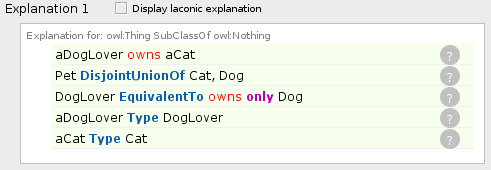
\includegraphics[trim = 0mm 0mm 0mm 0mm, clip, scale=0.65]{./ExplanationForDogLoverWithCat.png}
      \caption{Explanation for \texttt{DogLover} with a cat}\label{fig_ExplanationForDogLoverWithCat}
    \end{figure}

  
  \section{A Serious Flaw}
  To keep our ontology as simple as possible for this section, please remove any individuals you may have added to your ontology, but leave the \texttt{DogLover} class as we have defined it in the previous section. Just to ensure that our ontology is consistent, you run the reasoner to confirm that it is consistent. What we now want to do is to infer that when an individual owns something, that individual is a person. The way we can achieve this is by defining the domain for the \texttt{owns} property:
\begin{small}
\begin{verbatim} 
ObectProperty: owns
  Domain: Person
\end{verbatim}
\end{small}  
    \begin{figure}
    %trim option's parameter order: left bottom right top
      \centering 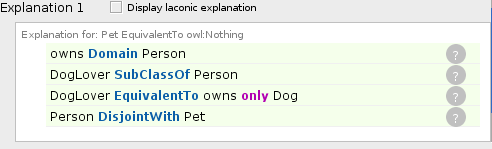
\includegraphics[trim = 0mm 0mm 0mm 0mm, clip, scale=0.65]{./ExplanationForPetEquivalentToNothing.png}
      \caption{Explanation for \texttt{Pet} equivalent to \texttt{owl:Nothing}}\label{fig_ExplanationForPetEquivalentToNothing}
    \end{figure}
    
Now, this looks like a rather innocent change, but when you run the reasoner again you will find that \texttt{Pet}, \texttt{Cat} and \texttt{Dog} are all equivalent to \texttt{owl:Nothing} while \texttt{Person} is equivalent to \texttt{owl:Thing}.
An explanation for why \texttt{Pet} is equivalent to \texttt{owl:Nothing} is given in Figure~\ref{fig_ExplanationForPetEquivalentToNothing}.

The explanation given in Figure~\ref{fig_ExplanationForPetEquivalentToNothing} can be difficult to understand. Indeed, research has shown that there are explanations that are difficult to understand even for experienced ontology designers~\cite{Horridge2011,Horridge2013}. In cases where it is hard to understand explanations, using laconic explanations can be helpful. Laconic justifications aim to remove subexpressions from axioms that do not contribute to explaining an entailment or inconsistency~\cite{Horridge2011,Horridge2013}. Ticking the ``Display laconic explanation'' displays the laconic explanation in Figure~\ref{fig_LaconicExplanationForPetEquivalentToNothing}.

The main difference between the explanations in Figures~\ref{fig_ExplanationForPetEquivalentToNothing} and \ref{fig_LaconicExplanationForPetEquivalentToNothing} are 

\begin{small}
\begin{verbatim} 
DogLover EquivalentTo owns only Dog
\end{verbatim}
\end{small}

versus

\begin{small}
\begin{verbatim} 
owns only owl:Nothing SubClassOf DogLover
\end{verbatim}
\end{small}

    \begin{figure}
    %trim option's parameter order: left bottom right top
      \centering 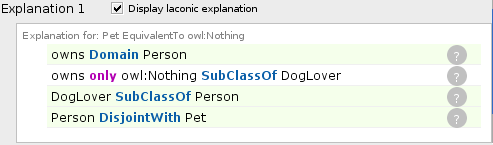
\includegraphics[trim = 0mm 0mm 0mm 0mm, clip, scale=0.65]{./LaconicExplanationForPetEquivalentToNothing.png}
      \caption{Laconic explanation for \texttt{Pet} equivalent to \texttt{owl:Nothing}}\label{fig_LaconicExplanationForPetEquivalentToNothing}
    \end{figure}


Where does \texttt{owns only owl:nothing SubClassOf DogLover} come from? Recall that \texttt{A EquivalentTo B} is just syntactical sugar for the two axioms \texttt{A SubClassOf B} and \texttt{B SubClassOf A}. What this explanation is saying is that there is a problem with the \texttt{owns only Dog SubClassOf DogLover} part of our axiom (there is no problem with the \texttt{DogLover SubClassOf owns only Dog} part of our axiom). Furthermore, it states that \texttt{Dog} is inferred to be equivalent to \texttt{owl:Nothing}. For this we need to understand the meaning of \texttt{owns only Dog} better. 

In Figure~\ref{fig_OwnsOnlyDog} I give an example domain where I make the assumption that for all individuals all ownership information is specified explicitly. Thus, individuals with no ownership links own nothing and individuals with ownership links own only what is specified and nothing else. The \texttt{owns only Dog} class includes all individuals that are known to own nothing besides dogs. However, a confusing aspect of the semantics of universal restrictions is that it also includes those individuals that owns nothing. To confirm this for yourself you can use the following ontology (from which I removed the domain restriction for the moment). This ontology will infer that \texttt{anIndividualOwningNothing} is of type \texttt{DogLover}.

\begin{small}
\begin{verbatim} 
ObjectProperty: owns
        
Class: Cat
  SubClassOf: Pet
    
Class: Dog
  SubClassOf: Pet
    
Class: Person
  DisjointWith: Pet
        
Class: Pet
  DisjointUnionOf: Cat, Dog
  DisjointWith: Person
  
Class: DogLover
  SubClassOf: Person
  owns only Dog SubClassOf: DogLover
  
Individual: anIndividualOwningNothing
  Types: owns only (not owl:Thing)
\end{verbatim}
\end{small} 

We are now ready to explain why \texttt{Pet} is equivalent to \texttt{owl:Nothing}:
\begin{enumerate}
 \item \texttt{owns Domain Person} states that whenever an individual owns something, that individual is a \texttt{Person}. 
 \item \texttt{owns only Pet SubClassOf DogLover} includes saying that when an individual owns nothing at all, that individual is a \texttt{DogLover}.
 \item Since \texttt{DogLover} is a subclass of \texttt{Person} it means \texttt{Person} now includes individuals that owns something and individuals that owns nothing, which means \texttt{Person} is equivalent to \texttt{owl:Thing}.
 \item \texttt{Person} and \texttt{Pet} are disjoint, hence \texttt{Pet} must be equivalent to \texttt{owl:Nothing}.
\end{enumerate}

    \begin{figure}
    %trim option's parameter order: left bottom right top
      \centering 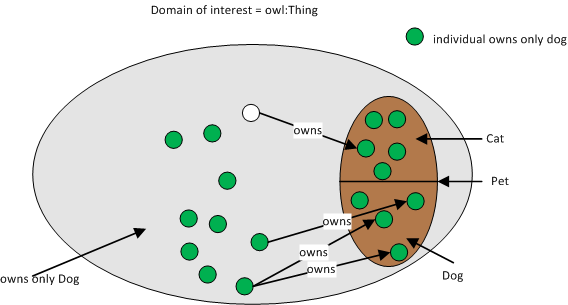
\includegraphics[trim = 0mm 0mm 0mm 0mm, clip, scale=1]{./OwnsOnlyDog.png}
      \caption{The meaning of \texttt{owns only Dog}}\label{fig_OwnsOnlyDog}
    \end{figure}

  \section{Conclusion} 
So how do we fix our ontology? Simple, we enforce that for someone to be a \texttt{DogLover}, they must own at least 1 dog and nothing else but dogs.  
\begin{small}
\begin{verbatim} 
Class: DogLover
  EquivalentTo: owns some Dog and owns only Dog
\end{verbatim}
\end{small}   

The example ontologies of this post can be found in \href{https://github.com/henrietteharmse/henrietteharmse/tree/master/blog/tutorial/ontologies/docs/Understanding%20OWL%20Universal%20Property%20Restrictions}{github}.

  \bibliographystyle{amsplain}
  \bibliography{./BibliographicDetails_v.0.1}
 
\end{document}
